\documentclass{report}
\usepackage[utf8]{inputenc}
\usepackage{amsmath}
\usepackage{graphicx}

\title{Eksamensnoter - Divide and Conquer}
\author{André Oskar Andersen (wpr684)}
\date{\today}

\begin{document}
\maketitle

\section*{15 Dynamic Pgoramming}
\begin{itemize}
    \item Dynamic programming, like the divide-and-conquer method, solves problems by dombining the solutions to subproblems. Dynamic programming applies when the subproblems overlap - that is, when subproblems share subsubproblems. A dynamic-programming algorithm solves each subsubproblem just once and then saves its answer in a table, thereby avoiding the work of recomputing the answer every time it solves each subsubproblem
\end{itemize}

\subsection*{15.1 Rod cutting}
\begin{itemize}
    \item Our first example uses dynamic programming to solve a simple problem in deciding where to cut steel rods. Serling Enterprises buys long steel rods and cuts them into shorter rods, which it then sells. Each cut is free. The management of Serling Enterprises wants to know the best way to cut up the rods
    \item We assume that we know for $i = 1, 2, ...$ the price $p_i$ in dollars that Serling Enterprises charges for a rod of length \textit{i} inches.
    \item The \textit{rod-cutting problem} is as following. Given a rod of length \textit{n} inches and a table of prices $p_i$ for $i = 1, 2, ..., n$, determine the maximum revenue $_n$ obtainable by cutting up the rod and selling the pieces. We can cut up a rod of length \textit{n} in $2^{n - 1}$ different ways, since we have an independent option of cutting, or not cutting, at distance \textit{i} inches from the left end, for $i = 1, 2, ..., n - 1$. If an optimal solution cuts the rod into \textit{k} pieces, for some $1 \leq k \leq n$, then an optimal decomposition $n = i_1 + i_2 + ... + i_k$ of the rod into pieces of length $i_1, i_2, ..., i_k$ provides maximum corresponding revenue $r_n = p_{i_1} + p_{i_2} + p_{i_k}$. 
    More generally, we can frame the values $r_n$ for $n \geq 1$ in terms of optimal revenues fro mshorter rods: 
    $$r_n = \max(p_n, r_1 + r_{n - 1}, r_2 + r_{n - 2}, ..., r_{n - 1} + r_1)$$
    The first argument, $p_n$, corresponds to making no cuts at all and selling the rod of length \textit{n} as is. The other $n - 1$ arguments to max correspond to the maximum revenue obtained by making an initial cut of the rod into two pieces of size \textit{i} and $n - i$, for each $i = 1, 2, ..., n - 1$, and then optimally cutting up those pieces further, obtaining revenues $r_i$ and $r_{n - 1}$ from those two pieces.
    We say that the rod-cutting problem exhibits \textit{optimal substructure}: optimal solutions to a problem incorporate optimal solutions to related subproblems, which we may solve independently.
    In a related way to arrange a recursive structure for the rod-cutting problem, we view a decomposition as consisting of a first piece of length \textit{i} cut off the left-hand end, and then a right-hand remainder of length $n - i$. Only the remainder, and not the first piece, may be further divided. We thus obtain the following simpler equation:
    $$r_n = \max_{1 \leq i \leq n} (p_i + r_{n - i})$$
    In this formulation, an optimal solution embodies the solution to only one related subproblem - the remainder - rather than two.
\end{itemize}
\textbf{Recursive top-down implementation}
\begin{itemize}
    \item There are $2^{n - 1}$ ways of cutting up \textit{R}, hence the this algorithm runs in exponential time
\end{itemize}
\textbf{Using dynamic programming for optimal rod cutting}
\begin{itemize}
    \item The dynamic-programming method works as follows. Having observed that anaive recursive solution is inefficient because it solves the same subproblems repeatedly, we arrange for each ubproblem to be solved only once, saving its solution. If we need to refer to this subproblem's solution again later, we can just look it up, rather than recompute it.
    \item There are usually two equivalent ways to implement a dynamic-programming approach:
    \begin{enumerate}
        \item The first approach is \textit{top-down with memoization}. In this approach, wewrite the procedure reursively in a natural manner, but modified to save the result of each subproblem. The procedure now first checks to see whether it has previously solved this subproblem. If so, it returns the saved value, saving further computation at this level; if not, the procedure computes the value in the usual manner. We say that the recursive procedure has been \textit{memoized}; it "remembers" what results it has computed previously
        \item The second approach is the \textit{bottom-up method}. This approach typically depends on some natural notion of the "size" of a subproblem, such that solving any particular subproblem depends only on solving "smaller" subproblems. We sort the subproblems by size and solve them in size order, smallest first. When solving a particular subproblem, we have already solved all of the smaller subproblems its solution depends upon, and we have saved their solutions. We solve each subproblem only once, and when we first see it, we have already solved all of its prerequisite subproblems.
    \end{enumerate}
    \item The two approaches have the same asymptotic running time; $\Theta(n^2)$
\end{itemize}
\textbf{Subproblem graph}
\begin{center}
    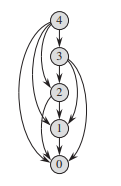
\includegraphics[height = 5 cm]{../entities/subproblem_graph.png}
\end{center}
\begin{itemize}
    \item The \textit{subproblem graph} for the problem embodies the set of subproblems involved and how subproblems depend on one another
    \item It is a directed graph, containing one vertex for each distinct subproblem. The subproblem graph has a directed edge from the vertex for subproblem \textit{x} to the vertex for subproblem \textit{y} if determining an optimal solution for subproblem \textit{x} involves directly considering an optimal solution for subproblem \textit{y}.
    \item The size of the subproblem graph $G = (V, E)$ can help us determine the running time of the dynamic programming algorithm. Since we solve each subroblem just once, the running time is the sum of the times needed to selve each subproblem. Typically, the time to compute the solution to a subproblem is proportional to the out-degree (number of outgoing edges) of the corresponding vertex in the subproblem graph, and the number of subproblems is equal to the number of vertices in the subproblem graph. In this common case, the running time of dynamic programming is linear in the number of vertices and edges
\end{itemize}

\subsection*{15.3 Elements of dynamic programming}
\begin{itemize}
    \item The two key ingredients that an optimization problem must have in order for dynamic programming to apply are optimal substructure and overlapping subproblems.
\end{itemize}
\textbf{Optimal substructure}
\begin{itemize}
    \item The first step in solving an optimization problem by dynamic programming is to characterize the structure of an optimal solution. Recall that a problem exhibits \textit{optimal substructure} if an optimal solution to the problem contains within it optimal solutions to subproblems. Whenever a problem exhibits optimal substructure, we have a good clue that dynamic programming might apply. in dynamic programming, we build an optimal solution to the problem from optimal solutions to subproblems.
    \item In Section 15.1, we observed that the optimal way of cutting up a rod of length \textit{n} involves optimally cutting up the two pieces resulting from the first cut.
    \item An optimal solution to the whole problem consists of optimal solutions to subproblems which can be solved independently
\end{itemize}

\textbf{Overlapping subproblems}
\begin{itemize}
    \item The second ingredient that an optimization problem must have for dynamic programming to apply is that the space of subproblems must be "small" in the sense that a recursive algorithm for the problem solves the same subproblems over and over, rather than always generating new subproblems. When a recursive algorithm revisits the same problem repeatedly, we say that the optimization problem has \textit{overlapping subproblems}
\end{itemize}

\textbf{Memoization}
\begin{itemize}
    \item There is an alternative approach to dynamic programming that often offers the efficiency of the obttom-up dynamic-programming approach while maintaining a top-down strategy. The idea is to \textit{memoize} the natural, but inefiicient, recursive algorithm. As in the bottom-up approach, we maintain a table with subproblem solutions, but the control structure for filling in the table is more like the recursive algorithm
    \item A memoized recursive algorithm maintains an entry in a table for the solution to each subproblem. When the subproblem is first encountered as recursive algorithm unfolds, its solution is computed and then stored in the table. Each subsequent time that we encounter this subproblem, we simply look up the value stored in the table and return it
    \item In general practive, if all subproblems must be solved at least once, a bottom-up dynamic-programming algorithm usually outperforms the correpsonding top-down memoized algorithm by a constant factor, because the bottom-up algorithm has no overhead for recursion and less overhead for maintaining the table. Moreover, for some problems we can exploit the regular pattern of table accesses in the dynamic-programming algorithm to reduce time or space requirements even further. Alternatively, if some subproblems in the subproblem space need not be solved at all, the memoized solution has the advantage of solving only those subproblems that are definitely required.
\end{itemize}

\subsection*{15.4 Longest common subsequence}
\begin{itemize}
    \item A strand of DNA consists of a string of molecules called \textit{bases}. We can express a strand of DNA as a string over the finite set $\{A, C, G, T\}$. We measure the similarity of to strands, $S_1$ and $S_2$ by finding a third strand $S_3$ in which the bases in $S_3$appear in each of $S_1$and $S_2$; these bases must appear in the same order, but not necessarily consecutively. The longer the strand $S_3$we can find, the more similar $S_1$and $S_2$ are.
    \item A subsequence of a given sequence is just the given sequence with zero or more elements left out. Formally, given a sequence $X = \{x_1, x_2, ..., x_m\}$, another sequence $Z = \{z_1, z_2, ..., z_k\}$ is a \textit{subsequence} of $X$ if there exists a strictly increasing sequence $\{i_1, i_2, ..., i_k\}$ of indices of $X$ such that for all $j = 1, 2, ..., k$, we have $x_{i_j} = z_j$.
    \item Given two sequences \textit{X} and \textit{Y}, we say that a sequence \textit{Z} is a \textit{common subsequence} of \textit{X} and \textit{Y} if \textit{Z} is a subsequence of both \textit{X} and \textit{Y}.
    \item In the \textit{longest-common-subsequence (LCS) problem}, we are given two sequences and wish to find a maximum-length common subsequence of these two sequences. This section shows how to efficiently solve the LCS problem using dynamic programming
\end{itemize}

\begin{center}
    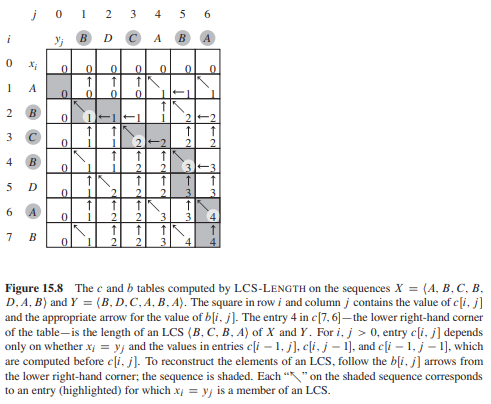
\includegraphics[height = 7 cm]{../entities/LCS_example.png}
\end{center}

\textbf{Step 1: Characterizing a longest common subsequence}
\begin{itemize}
    \item The LCS problem has an optimal-substructure property. Given a sequence $X = \{x_1, x_2, ..., x_m\}$, we define the \textit{i}th \textit{prefix} of \textit{X}, for $i = 0, 1, ..., m$, as $X_i = \{x_1, x_2, ..., x_i\}$. \\
    \textbf{Theorem 15.1 (Optimal substructure of an LCS}
    \begin{itemize}
        \item Let $X = \{x_1, x_2, ..., x_m\}$ and $Y = \{y_1, y_2, ..., y_n\}$ be sequences, and let $Z = \{z_1, z_2, ..., z_k\}$ be any LCS of \textit{X} and \textit{Y}.
        \begin{enumerate}
            \item If $x_m = y_n$, then $z_k = x_m = y_n$ and $Z_{k - 1}$ is an LCS of $X_{m - 1}$ and $Y_{n - 1}$
            \item If $x_m \neq y_n$, then $z_k \neq x_m$ implies that \textit{Z} is an LCS of $X_{m - 1}$ and $Y$
            \item If $x_m \neq y_n$, then $z_k \neq y_n$ implies that \textit{Z} is an LCS of $Y_{n - 1}$ and $X$
        \end{enumerate}
    \end{itemize}
    \textbf{Proof}
    \begin{enumerate}
        \item If $z_k \neq x_m$, then we could append $x_m = y_n$ to \textit{Z} to obtain a common subsequence of \textit{X} and \textit{Y} of length $k + 1$, contradicting the supposition that \textit{Z} is a longest common subsequence of \textit{X} and \textit{Y}. Thus, we must have $z_k = x_m = y_n$. Now, the prefix $Z_{k - 1}$ is a length-($k - 1$) common subsequence of $X_{m - 1}$ and $Y_{n - 1}$. We wish to show that it is an LCS. Suppose for the purpose of contradiction, that there exists a common subsequence $W$ of $X_{m - 1}$ and $Y_{n - 1}$ with length greater than $k - 1$. Then, appending $x_m = y_n$ to $W$ of $X_{m - 1}$ and $Y_{n - 1}$ with length greater than $k - 1$. Then appending $x_m = y_n$ to $W$ produces a common subsequence of $X$ and $Y$ whose length is greater than $k$, which is a contradiction
        \item If $z_k \neq x_m$, then $Z$ is a common subsequence of $X_{m - 1}$ and $Y$. If there were a common subsequence $W$ of $X_{m - 1}$ and $Y$ with length greater than $k$, then $W$ would also be a common subsequence of $X_m$ and $Y$, contradicting the assumption that $Z$ is an LCS of $X$ and $Y$
        \item The prrof is symmetric to case 2
    \end{enumerate}
    \item The way that Theorem 15.1 characterizes longest common subsequences tells us that an LCS of two sequences contains within it an LCS of prefixes of the two sequences. Thus, the LCS problem has an optimal-substructure property.
\end{itemize}
\textbf{Step 2: A recursive solution}
\begin{itemize}
    \item Theorem 15.1 implies that we should examine either one or two subproblems when finding an LCS of $X = \{x_1, x_2, ..., x_m\}$ and $Y = \{y_1, y_2, ..., y_n\}$. If $x_m = y_n$, we must find an LCS of $X_{m - 1}$ and $Y_{n - 1}$. Appending $x_m = y_n$ to this LCS yields an LCS of $X$ and $Y$. If $x_m \neq y_n$, then we must solve two subproblems: finding an LCS of $X_{m - 1}$ and $Y$ and finding an LCS of $X$and $Y_{n - 1}$. Whichever of these two LCSs is longer is an LCS of $X$ and $Y$. Because these cases exhault all possibilities, we know that one of the optimal subproblem solutions must appear within an LCS of $X$ and $Y$
    \item We can readily see the overlapping-subproblems property in the LCS problem. To find a LCS of $X$ and $Y$, we may need to find the LCSs of $X$ and $Y_{n - 1}$ and of $X_{m - 1}$ and $Y$. But each of these subproblems has the subsubproblem of finding and LCS of $X_{m - 1}$ and $Y_{n - 1}$. Many other subproblems share subsubproblems.
    \item The recursive solution to the LCS problem involves establishing a recurrence for the value of an optimal solution. Let $c[i, j]$ be the length of an LCS of the sequences $X_i$ and $Y_j$. If either $i = 0$or $j = 0$, one of the sequences has length 0, and so the LCS has length 0. The optimal substructure of the LCS problem gives the recursive formula
    \[
        c[i, j] =
        \begin{cases}
            0 & \text{if $i = 0$ or $j = 0$} \\
            c[i - 1, j - 1] + 1 & \text{if $i, j > 0$ and $x_i = y_i$} \\
            \max(c[i, j - 1], c[i - 1, j]) & \text{if $i, j > 0$ and $x_i \neq y_j$}
        \end{cases}
    \]
\end{itemize}
\textbf{Step 3: Computing the length of an LCS}
\begin{itemize}
    \item Based on the equation for $c[i ,j]$, we could easily write an exponential-time recursive algorithm to compute the length of an LCS of two sequences. Since the LCS problem has only $\Theta(nm)$ distinct subproblems, however, we can use dynamic programming to compute the solutions bottom up
    \item The procedure takes two sequences, $X$ and $Y$, as inputs. It stores the $c[i, j]$ values in a table $c[0...m, 0...n]$, and it computes the entries in \textit{row-major} order (left to right, then the next row, and so on...).The procedure also maintains the table $b[1...m, 1..n]$ to help us construct an optimal solution. Intuitively, $b[i, j]$ points to the table entry corresponding to the optimal subproblem solution chosen when computing $c[i, j]$. The procedure reutrn the $b$ and $c$ tables; $c[m, n]$ contains the length of an LCS of $X$ and $Y$
\end{itemize}
\textbf{Step 4: Constructing an LCS}
\begin{itemize}
    \item The \textit{b} table returned by LCS-LENGTH enables us to quickly construct an LCS of $X$ and $Y$. We simply begin at $b[m, n]$ and trace through the table by following the arrows. Whenever we encounter a diagonal array, pointing top right, in entry $b[i, j]$, it implies that $x_i = y_j$ is an element of the LCS that LCS-LENGTH found.
    \item The procedure for printing out an LCS $X$ and $Y$ in the proper, forward oder, takes time $O(m + n)$, since it decrements at least one of $i$and $j$ in each recursive call
\end{itemize}

\end{document}